\documentclass[conference]{IEEEtran}

\usepackage[utf8]{inputenc}
\usepackage[T1]{fontenc}
\usepackage[spanish,es-noshorthands]{babel}
\usepackage{graphicx}
\graphicspath{{main_ASADA_images/}{Tecnologia_en_Marcha/main_ASADA_images/}}
\usepackage{array}
\usepackage{tabularx}
\usepackage{booktabs}
\usepackage{url}
\usepackage{cite}
\usepackage{tikz}
\usetikzlibrary{arrows.meta,positioning}

\urlstyle{same}
\renewcommand{\IEEEkeywordsname}{Palabras clave}
\renewcommand{\abstractname}{Resumen}
\sloppy

\title{Digitalización de acueductos rurales gestionados por comunidades en Costa Rica:\\ Una síntesis calibrada por evidencia de tres desarrollos de prototipos}

\author{
\IEEEauthorblockN{María José Angulo Campos}
\IEEEauthorblockA{
\textit{Tecnológico de Costa Rica}\\
Cartago, Costa Rica \\
https://orcid.org/0009-0005-5842-1101}
\and
\IEEEauthorblockN{Carlos Montoya Marín}
\IEEEauthorblockA{
\textit{Tecnológico de Costa Rica}\\
Cartago, Costa Rica \\
https://orcid.org/0009-0001-1561-9768}
\and
\IEEEauthorblockN{Juan José Montero-Jiménez}
\IEEEauthorblockA{
\textit{Tecnológico de Costa Rica}\\
Cartago, Costa Rica \\
https://orcid.org/0000-0002-3215-3736}
\and
\IEEEauthorblockN{Juan José Rojas-Hernández}
\IEEEauthorblockA{
\textit{Tecnológico de Costa Rica}\\
Cartago, Costa Rica \\
https://orcid.org/0000-0002-3261-5005}
}

\begin{document}
\maketitle

\begin{abstract}
Este artículo presenta una síntesis retrospectiva de casos múltiples de tres prototipos de monitoreo digital desarrollados con acueductos rurales gestionados por comunidades (ASADAS) en Costa Rica: Las Juntas de Abangares, Playa Sámara y Paso Ancho--Boquerón. El estudio pregunta cuáles necesidades operativas y funciones lógicas recurren entre los casos, cómo las restricciones del sitio modifican su implementación física y qué evidencia respalda la transferencia hacia futuros despliegues. Se aplicó un marco de extracción predefinido a informes técnicos, proyectos de graduación y artefactos de diseño versionados. La evidencia se clasificó desde trabajo planificado (E0) hasta operación sostenida en campo (E4) para evitar tratar cálculos, pruebas de banco y verificaciones de campo limitadas como equivalentes. La síntesis identifica una cadena funcional reutilizable---medición, adquisición y validación local, comunicación, servicios de datos e información para el operador---con energía, seguridad, monitoreo de salud y mantenibilidad como preocupaciones transversales. Una arquitectura de referencia configurable y criterios de decisión de sitio a módulo explicitan qué funciones permanecen estables y qué componentes deben cambiar según la instrumentación, la energía, la cobertura, la distancia y la capacidad de mantenimiento. Los casos respaldan la factibilidad funcional de subsistemas seleccionados, pero ninguno aporta evidencia E4. Por lo tanto, la arquitectura es una hipótesis de diseño trazable y no una solución universal validada en campo; la disponibilidad, la autonomía energética, el desempeño de alertas, la aceptación de operadores, los costos y los efectos sobre pérdidas de agua o continuidad del servicio requieren despliegue sostenido.
\end{abstract}

\begin{IEEEkeywords}
sistemas de agua gestionados por comunidades, acueductos rurales, ASADA, Internet de las cosas, monitoreo remoto, MBSE, arquitectura modular, síntesis de casos
\end{IEEEkeywords}

\section{Introducción}

La transformación digital en la infraestructura hídrica combina sensado, comunicaciones, gestión de datos y automatización dentro de un sistema operativo \cite{arnell2023making,zulkifli2022iot,velayudhan2022iot}. En entornos con recursos restringidos, el monitoreo remoto puede reducir los retrasos de información, pero la operación exitosa depende de más que conectar un sensor a un servicio en la nube. La compatibilidad de modernización, la autonomía energética, la conectividad intermitente, la mantenibilidad y la capacidad de los operadores para actuar con base en la información son igualmente importantes. Estudios previos han demostrado el monitoreo remoto de bombas manuales rurales y nodos de modernización con energía solar \cite{thomson2012gsm,bawankar2024iot}; sin embargo, la transferencia de estas soluciones sigue dependiendo de la infraestructura local y de los arreglos de servicio.

Costa Rica cuenta con más de 2000 organizaciones comunitarias de agua, conocidas como ASADAS, que gestionan sistemas locales de agua potable \cite{direccion2025asadas}. Estudios previos han documentado limitaciones en la condición de la infraestructura, el mantenimiento y la capacidad técnica de los prestadores rurales \cite{soto2016situacion,gaviria2020risk}. En este contexto, el Laboratorio Delta del Tecnológico de Costa Rica participó en una secuencia de prototipos que avanzó desde la adquisición autónoma de nivel de tanque hasta la integración distribuida de medidores y las interfaces industriales \cite{chavarria2021implementacion,solorzano2021sistema,oviedo2024desarrollo}. Un artículo relacionado de ISSE 2025 formalizó una arquitectura genérica para sistemas IoT de acueductos rurales mediante ARCADIA e ingeniería de sistemas basada en modelos (MBSE) \cite{arguedas2025towards}.

El presente artículo no afirma una nueva validación en campo de esa arquitectura. Su contribución distintiva es una reconstrucción calibrada por evidencia de los tres desarrollos previos. En contraste con \cite{arguedas2025towards}, que presenta la arquitectura MBSE genérica, este estudio: (i) incluye Las Juntas de Abangares; (ii) aplica un único marco de extracción comparativa a los tres casos; (iii) separa funciones planificadas, simuladas, probadas en banco, probadas en campo y sostenidas; y (iv) convierte los hallazgos transversales en criterios explícitos de configuración y verificación. El análisis aborda tres preguntas de investigación:

\begin{description}
\item[RQ1:] ¿Qué necesidades operativas y funciones lógicas recurren en los tres desarrollos?
\item[RQ2:] ¿Cómo cambian las restricciones del sitio la implementación física mientras la cadena funcional permanece estable?
\item[RQ3:] ¿Qué nivel de evidencia respalda cada capacidad y qué debe verificarse antes de transferirla a otra ASADA?
\end{description}

Este encuadre limita deliberadamente la inferencia a los casos documentados. ``Recurrente'' significa observado en al menos dos casos; no significa universal entre las ASADAS costarricenses. Del mismo modo, ``transferibilidad'' denota condiciones explícitas de adaptación y evaluación, no desempeño demostrado en un sitio no estudiado.

\section{Método}

\subsection{Diseño del estudio y límites de los casos}

Se realizó una síntesis retrospectiva de casos múltiples siguiendo la lógica de comparación de estudios de caso acotados \cite{yin2018case}. La unidad de análisis fue un desarrollo documentado de monitoreo digital asociado con una ASADA costarricense. Los casos se seleccionaron intencionalmente porque forman una secuencia de desarrollo trazable del mismo laboratorio y en conjunto cubren: (a) monitoreo autónomo del nivel de tanque, (b) monitoreo distribuido mediante medidores existentes y (c) interfaces analógicas y digitales industriales. La muestra disponible es, por tanto, útil analíticamente, pero no es aleatoria ni representativa de todas las ASADAS.

Las fuentes primarias fueron los proyectos finales de graduación e informes técnicos de Las Juntas de Abangares, Playa Sámara y Paso Ancho--Boquerón \cite{chavarria2021implementacion,solorzano2021sistema,oviedo2024desarrollo}. Dos fuentes complementarias tuvieron funciones más acotadas. El artículo de ISSE 2025 aportó la separación MBSE entre necesidades operativas, funciones lógicas y componentes físicos \cite{arguedas2025towards}. Un repositorio versionado de 2026 aportó el estado de la implementación actual de Paso Ancho \cite{deltalabo2026repo}. Debido a que ese repositorio representa una iteración posterior de diseño, se reporta por separado y no se contabiliza como un cuarto caso validado.

\subsection{Extracción y análisis transversal de casos}

El mismo marco de extracción se aplicó a cada caso:
\begin{enumerate}
\item Contexto y requisitos: problema operativo, usuarios, activos, necesidades de muestreo, restricciones ambientales, energía y conectividad.
\item Proceso de ingeniería: descomposición funcional, alternativas, criterios de selección, pasos de integración, revisiones motivadas por pruebas e interfaces no resueltas.
\item Implementación: variables, sensores, controladores, protocolos, suministro de energía, servicios de datos, alarmas y funciones orientadas al control.
\item Evidencia: entorno de prueba, medición de referencia, resultado reportado, función respaldada y verificación pendiente.
\end{enumerate}
Los detalles ausentes en una fuente se marcaron como no reportados, en lugar de inferirse. El análisis primero resumió cada caso y luego comparó los campos codificados entre casos. Una necesidad se marcó como recurrente entre casos cuando el mismo propósito operativo apareció en al menos dos desarrollos. Los requisitos específicos de un sitio se conservaron como restricciones. Luego, las funciones lógicas se mapearon a alternativas físicas sin tratar un componente usado una sola vez como preferible de manera universal.

No se calculó una estadística de confiabilidad entre codificadores; esta es una limitación de la síntesis retrospectiva. Para hacer auditable la interpretación, el manuscrito cita secciones de las fuentes, separa el repositorio posterior de los tres casos y proporciona una matriz de evidencia y trazabilidad en la Tabla~\ref{tab:evidence}.

\subsection{Calibración de la evidencia}

Para evitar que pruebas distintas se interpretaran como equivalentes, a cada capacidad reportada se le asignó el nivel más alto respaldado por su fuente:
\begin{itemize}
\item E0: requisito, diseño o verificación planificada únicamente;
\item E1: cálculo o simulación;
\item E2: prueba de componente o de banco;
\item E3: prueba de campo limitada o prueba parcial de extremo a extremo;
\item E4: operación sostenida en campo con duración y métricas de desempeño definidas.
\end{itemize}
La escala describe la solidez de la evidencia, no la madurez tecnológica en general. Para este artículo no se realizaron nuevas mediciones, entrevistas, pruebas prolongadas ni análisis estadísticos.

\section{Evidencia de los casos}

\subsection{Las Juntas de Abangares}

CIEDES requería registros de nivel de tanque para estudios de balance hídrico, demanda y capacidad de suministro. El nivel se había medido aproximadamente cada quince días y se registraba manualmente. Los requisitos incluían mediciones con marca temporal cada hora o cada 20 minutos, consultas remotas, gráficos, descargas y operación sin conexión a la red eléctrica \cite[Secs.~4.1--4.3]{chavarria2021implementacion}.

El diseño comparó arreglos HTTP y MQTT, así como alternativas de sensado, control y energía. HTTP se seleccionó por su integración simple a la frecuencia requerida. Retrasos de conexión y fallas de comandos con el SIM900 motivaron su reemplazo por un módem SIM7600, mientras que la conmutación temporizada de energía redujo el consumo \cite[Secs.~4.4--5.1]{chavarria2021implementacion}. El prototipo integró un sensor ultrasónico AJ-SR04, Arduino Nano, reloj de tiempo real, módem celular, base de datos web y suministro solar. Comparaciones con cinta métrica respaldaron la calibración del sensor; pruebas funcionales respaldaron la transmisión, el almacenamiento, la consulta, el graficado y la descarga. La autonomía energética se respaldó mediante cálculos de dimensionamiento y simulación fotovoltaica, no mediante observación sostenida en campo.

\subsection{Playa Sámara}

Este caso buscó información hidráulica distribuida y coordinación de bombeo, conservando medidores ARAD Octave. Las restricciones incluyeron activos dispersos, operación sin red eléctrica, humedad, corrosión y un intervalo de reporte refinado para acomodar el servicio MQTT seleccionado \cite[Secs.~1.3--2.1]{solorzano2021sistema}. El diseño separó funciones de comunicación, medición y orientación al control. Las pruebas del medidor llevaron a revisar la interpretación de pulsos y la resolución antes de las verificaciones finales.

Tres dispositivos basados en ESP32 adquirieron pulsos SSR de Octave y combinaron energía solar, enlaces LoRa, una puerta de enlace, MQTT y Adafruit IO. El informe usa terminología LoRaWAN; la descripción disponible respalda directamente enlaces LoRa con una puerta de enlace y paquetes de aplicación. Las comparaciones referenciadas al despliegue del medidor produjeron 0\% de diferencia en volumen acumulado y 0.72\% o 0.73\% de diferencia en caudal promedio, según la sección del informe \cite[Sec.~5.2.2 y conclusiones]{solorzano2021sistema}. Esta discrepancia interna, la ausencia de exactitud de referencia absoluta y la modificación de bombeo no instalada limitan el alcance de la afirmación a funciones de adquisición y comunicación probadas.

\subsection{Paso Ancho--Boquerón (2024)}

El acceso difícil a los tanques motivó el monitoreo remoto de nivel, caudal y volumen, conservando medidores Octave compatibles. Los requisitos separaron arquitectura del nodo, integración de mediciones, integración de la puerta de enlace y visualización \cite[Secs.~1.3--2.1]{oviedo2024desarrollo}. Un M-Duino 21+LoRa adquirió una señal de nivel acondicionada de 4--20~mA y registros Octave mediante Modbus. La energía solar alimentó el nodo; LoRa lo conectó con una puerta de enlace y WiFi conectó la puerta de enlace con ThingSpeak.

Las verificaciones de campo respaldaron la adquisición Modbus. La integración posterior en el TEC usó un tanque representativo para el nivel y la comunicación nodo--puerta de enlace. Debido a que allí no había disponible un medidor Octave compatible, la visualización de extremo a extremo usó lecturas de campo previas y valores asumidos de caudal y volumen \cite[Sec.~6.2 y anexos~9.2--9.3]{oviedo2024desarrollo}. Por tanto, la evidencia respalda integración parcial, no operación sostenida de la cadena completa.

\begin{table*}[t]
\caption{Evidencia y trazabilidad en los tres casos.}
\label{tab:evidence}
\centering
\scriptsize
\renewcommand{\arraystretch}{1.12}
\begin{tabularx}{\textwidth}{@{}>{\raggedright\arraybackslash}p{0.14\textwidth}>{\raggedright\arraybackslash}X>{\raggedright\arraybackslash}p{0.12\textwidth}>{\raggedright\arraybackslash}X>{\raggedright\arraybackslash}X@{}}
\toprule
\textbf{Caso y fuente} & \textbf{Evidencia máxima respaldada} & \textbf{Nivel} & \textbf{Funciones respaldadas} & \textbf{Límite principal para la síntesis} \\
\midrule
Las Juntas \cite{chavarria2021implementacion} & Calibración, verificaciones funcionales de la cadena web y pruebas de hardware de energía; dimensionamiento y simulación de energía & E3 para funciones limitadas; E1 para autonomía & Adquisición de nivel, HTTP celular, almacenamiento, consulta, gráficos y descargas & Duración, disponibilidad en campo y autonomía energética de largo plazo no reportadas \\
Playa Sámara \cite{solorzano2021sistema} & Pruebas de banco y campo limitadas de la interfaz con medidor, firmware, enlace de radio y servicio de datos & E3 & Adquisición de pulsos, ruta LoRa/puerta de enlace, servicio MQTT y lógica de alarmas & Comparación referenciada al despliegue; discrepancia de caudal; actuación no instalada; sin registro sostenido \\
Paso Ancho--Boquerón \cite{oviedo2024desarrollo} & Verificación Modbus en campo e integración parcial en el TEC & E3 & Entrada 4--20~mA, adquisición Modbus, recepción LoRa y demostración en la nube & Valores representativos o asumidos usados en la integración; sin operación sostenida de extremo a extremo \\
\bottomrule
\end{tabularx}
\end{table*}

\section{Hallazgos transversales}

\subsection{Necesidades recurrentes y funciones estables}

Cinco necesidades operativas recurrieron. Primero, la observabilidad remota reemplazó registros manuales intermitentes con datos con marca temporal. Segundo, la interoperabilidad preservó activos útiles mediante interfaces ultrasónicas, de pulsos, analógicas o Modbus. Tercero, la operación sin red eléctrica requirió arreglos seleccionables de energía y comunicación. Cuarto, los datos debían transformarse en gráficos accesibles, descargas, alarmas o información orientada al control. Quinto, la confiabilidad y la mantenibilidad requirieron calibración explícita, verificaciones de interfaz, salud del sistema, recuperación y configuración documentada.

En los tres casos, estas necesidades se mapean a una cadena lógica estable:
\begin{center}
\small medición $\rightarrow$ adquisición y validación local $\rightarrow$ comunicación\\
$\rightarrow$ almacenamiento y procesamiento $\rightarrow$ información para el operador.
\end{center}

La cadena es más estable que cualquier componente físico. Por ejemplo, HTTP puede reemplazarse por MQTT, LoRa por comunicación celular y un sensor ultrasónico por 4--20~mA o Modbus sin cambiar el propósito de la función lógica correspondiente.

\subsection{Arquitectura de referencia}

La Fig.~\ref{fig:architecture} convierte la comparación en una arquitectura de referencia configurable. Las flechas continuas muestran la ruta requerida desde la medición hasta la información. La banda superior contiene restricciones del sitio que determinan las opciones físicas. La banda inferior contiene requisitos transversales que deben verificarse entre módulos. Por tanto, la arquitectura no es una lista de materiales: es un conjunto de funciones estables, interfaces controladas e implementaciones seleccionables.

\begin{figure*}[t]
\centering
\resizebox{0.96\textwidth}{!}{%
\begin{tikzpicture}[
font=\scriptsize,
process/.style={draw=blue!80!black, line width=1.1pt, rounded corners=2pt, fill=blue!6, align=center, minimum height=1.15cm, text width=2.35cm, inner sep=3pt},
topband/.style={draw=orange!70!black, line width=0.7pt, rounded corners=2pt, fill=orange!12, align=center, minimum height=0.65cm, text width=14.7cm, inner sep=3pt},
bottomband/.style={draw=teal!60!black, line width=0.7pt, rounded corners=2pt, fill=teal!10, align=center, minimum height=0.75cm, text width=15.2cm, inner sep=3pt},
arrow/.style={-{Latex[length=2.2mm,width=2mm]}, draw=blue!80!black, line width=1pt}
]
\node[topband] (top) at (0,2.0) {Factores de configuración del sitio: instrumentación instalada, rango y frecuencia de medición, disponibilidad de\\energía, cobertura y distancia, ambiente, acceso, capacidad de mantenimiento y restricciones del servicio de datos};

\node[process] (m) at (-6.1,0.55) {1. Medición\\ultrasónico; pulsos;\\4--20~mA; Modbus};
\node[process] (e) at (-3.05,0.55) {2. Adquisición local\\marca temporal; escala;\\plausibilidad; búfer};
\node[process] (n) at (0,0.55) {3. Red de acceso\\LoRa + puerta de enlace;\\celular; WiFi};
\node[process] (d) at (3.05,0.55) {4. Servicios digitales\\ingesta; almac.; consulta;\\visualización; notificación};
\node[process] (o) at (6.1,0.55) {5. Operación\\estado; alarmas;\\decisiones; mantenimiento};

\draw[arrow] (m.east) -- (e.west);
\draw[arrow] (e.east) -- (n.west);
\draw[arrow] (n.east) -- (d.west);
\draw[arrow] (d.east) -- (o.west);

\node[bottomband] (bottom) at (0,-0.95) {Verificación transversal: autonomía energética, control de interfaces, calidad y trazabilidad de datos, disponibilidad\\y recuperación, ciberseguridad, protección ambiental, salud del sistema y mantenibilidad};

\draw[gray!55, line width=0.8pt, dash pattern=on 3pt off 4pt] (top.south) -- (e.north);
\draw[gray!55, line width=0.8pt, dash pattern=on 3pt off 4pt] (n.south) -- (bottom.north);
\end{tikzpicture}}
\caption{Arquitectura de referencia configurable derivada de la evidencia. Las funciones lógicas permanecen estables; las implementaciones físicas se seleccionan a partir de restricciones del sitio y se verifican de extremo a extremo.}
\label{fig:architecture}
\end{figure*}

\subsection{Criterios de configuración y verificación}

La Tabla~\ref{tab:criteria} operacionaliza la transferibilidad. No prescribe una tecnología única; en cambio, identifica la evidencia mínima de decisión requerida antes de replicar. Un módulo es transferible solo si se documentan su interfaz, los supuestos del sitio y sus criterios de aceptación.

\begin{table*}[t]
\caption{Criterios de decisión y verificación de sitio a módulo.}
\label{tab:criteria}
\centering
\scriptsize
\renewcommand{\arraystretch}{1.12}
\begin{tabularx}{\textwidth}{@{}>{\raggedright\arraybackslash}p{0.20\textwidth}>{\raggedright\arraybackslash}p{0.22\textwidth}>{\raggedright\arraybackslash}X>{\raggedright\arraybackslash}X@{}}
\toprule
\textbf{Condición observada del sitio} & \textbf{Decisión de configuración} & \textbf{Especificación requerida} & \textbf{Verificación mínima antes del despliegue} \\
\midrule
Medidor compatible o sensor industrial existente & Preservar el activo; seleccionar interfaz de pulsos, 4--20~mA o Modbus & Definición de registros/pulsos, rango, escalamiento, aislamiento, cableado y manejo de errores & Comparar contra una referencia trazable en el rango de operación; verificar desconexión, valores inválidos y comportamiento de recuperación \\
Sin energía fija & Nodo solar/batería con ciclos de trabajo & Perfil de carga, intervalo de muestreo/transmisión, objetivo de autonomía, recurso solar y gabinete & Prueba de carga en banco más balance energético; luego observar batería y disponibilidad del nodo bajo clima representativo \\
Nodos dispersos con acceso a puerta de enlace & Enlace local basado en LoRa & Distancia, terreno, carga útil, intervalo de reporte, política de paquetes y energía/retroconexión de la puerta de enlace & Levantamiento del sitio y prueba de entrega de paquetes en cada ubicación; verificar búfer y recuperación tras pérdida de enlace \\
Cobertura celular sin Internet local & Nodo celular directo & Operador/bandas, rango de señal, plan de datos, política de reintentos y consumo & Prueba de cobertura en las condiciones esperadas; carga de extremo a extremo, reintentos, búfer y recuperación tras ciclo de energía \\
El operador requiere alarmas o control & Agregar primero notificación; introducir actuación solo después de que el monitoreo sea confiable & Responsable del umbral, flujo de respuesta, estado seguro ante falla, autorización y pista de auditoría & Prueba de precisión y tiempo de entrega de alarmas; análisis de peligros de control y prueba de aceptación supervisada antes de la actuación \\
\bottomrule
\end{tabularx}
\end{table*}

\section{Iteración actual de Paso Ancho}

La aplicación actual de Paso Ancho es una instanciación posterior en desarrollo y no constituye evidencia de despliegue completado \cite{deltalabo2026repo}. Su documentación de misión incluye monitoreo móvil, alertas de rebalse y de suministro insuficiente, adquisición desde medidor Octave y sensor de nivel, operación sin energía ni Internet fijos, protección ambiental, mantenibilidad, disponibilidad y ciberseguridad.

La versión revisada inicializa RS-485, lee caudal y volumen mediante Modbus, escala una entrada analógica de altura a 0--5~m y emite resultados por un puerto serial. El contenedor SIM7600 está comentado, por lo que la transmisión LTE, la carga remota y la integración de extremo a extremo permanecen en E0. El sensor de profundidad One-Wire de 24~V documentado también difiere de la interfaz analógica implementada en firmware. Antes del despliegue, el equipo debería emitir un documento de control de interfaz que reconcilie el sensor físico, la conversión eléctrica, la entrada de firmware, las unidades de ingeniería, el rango, la resolución, los valores de falla y el procedimiento de calibración.

Las pruebas planificadas deberían cubrir la ruta completa de la Fig.~\ref{fig:architecture}, incluida la validación local, la transferencia sin Internet fijo, el almacenamiento, la visualización, las notificaciones, la salud del nodo, la recuperación, el control de acceso y el respaldo. Las afirmaciones de desempeño requerirán el firmware y la configuración desplegados, datos crudos, protocolos de prueba, criterios de aceptación definidos y duración de observación.

\section{Discusión}

\subsection{Qué se transfiere y qué no}

Los casos respaldan la transferencia de funciones lógicas con más fuerza que la transferencia de componentes. La observabilidad remota, la adquisición con marca temporal, una ruta de comunicación de extremo a extremo, datos persistentes, acceso para el operador y mantenibilidad son propósitos comunes. El tipo de sensor, el protocolo, el arreglo de energía, el controlador, la puerta de enlace y el servicio en la nube son decisiones dependientes del sitio. Esta distinción es el valor principal de la perspectiva MBSE: las necesidades operativas y el comportamiento lógico pueden conservarse mientras varían las implementaciones físicas \cite{arguedas2025towards,voirin2018arcadia}.

La modernización incremental puede preservar medidores Octave y otros activos útiles, lo que reduce reemplazos e interrupciones. La contraparte es una complejidad adicional en el acondicionamiento de señales, la interpretación de registros o pulsos, el control de versiones, la calibración y el diagnóstico de fallas. Del mismo modo, LoRa puede reducir el consumo energético de nodos de área amplia cuando existe una puerta de enlace mantenible y una retroconexión disponible, mientras que la comunicación celular puede eliminar la puerta de enlace, pero aumentar el consumo del nodo, la dependencia del servicio y el costo recurrente. La evidencia actual no establece una opción universalmente superior.

Los prototipos también muestran por qué el monitoreo, la lógica de decisión y la actuación deben verificarse por separado. La adquisición de datos puede ser funcional mientras las alarmas, la respuesta operativa o el control de bombeo permanecen sin probar. Introducir control antes de que la cadena de monitoreo haya demostrado marcas temporales, unidades, manejo de fallas, disponibilidad y recuperación confiables convertiría fallas de calidad de datos en peligros operativos.

\begin{figure}[t]
\centering
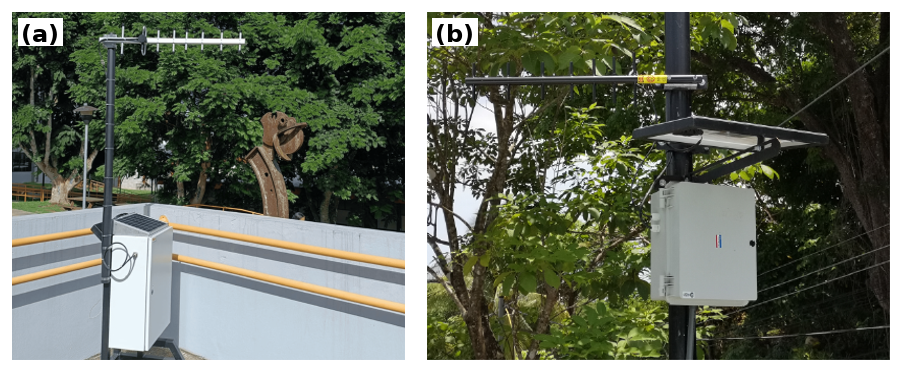
\includegraphics[width=\columnwidth]{figure-000.png}
\caption{Hardware representativo documentado: (a) Paso Ancho--Boquerón y (b) Playa Sámara \cite{solorzano2021sistema,oviedo2024desarrollo}. Las fotografías ilustran la variabilidad física y no una arquitectura invariante.}
\label{fig:hardware}
\end{figure}

\subsection{Límites de la evidencia y amenazas a la validez}

La síntesis tiene cuatro limitaciones principales. Primero, todos los casos se originaron en una misma línea institucional de desarrollo; el personal compartido y las preferencias de diseño reducen la independencia. Segundo, los informes fuente difieren en propósito, terminología, condiciones de prueba y nivel de detalle. Tercero, varias comparaciones usan despliegues de equipo, simulaciones, entradas representativas o valores asumidos, en lugar de instrumentos de referencia trazables y datos sostenidos de extremo a extremo. Cuarto, la codificación retrospectiva no fue replicada de manera independiente y no se realizaron entrevistas a actores para este artículo.

En consecuencia, los hallazgos respaldan un marco de diseño y factibilidad funcional bajo las condiciones de prueba reportadas, no una generalización poblacional. Ninguna fuente analizada establece disponibilidad sostenida, autonomía energética de largo plazo, carga de mantenimiento, desempeño de ciberseguridad, aceptación de operadores, costo-efectividad, reducción de pérdidas de agua o mejora de continuidad del servicio. Los criterios propuestos fortalecen la transferibilidad analítica, pero la transferencia empírica aún debe probarse en un sitio adicional.

\section{Agenda de evaluación operativa}

El próximo despliegue debería usar una matriz de verificación preregistrada que vincule cada requisito con una interfaz, prueba, criterio de aceptación, archivo de evidencia y rol responsable. Como mínimo, la evaluación sostenida debería reportar: disponibilidad de datos; registros faltantes y duplicados; integridad de marcas temporales y unidades; entrega de paquetes y recuperación tras interrupciones; estado de batería y autonomía; plausibilidad y deriva del sensor; precisión, recuperación y tiempo de entrega de alarmas; intervenciones de mantenimiento; finalización de tareas y aceptación por parte del operador; y costo de ciclo de vida. Las afirmaciones sobre pérdidas de agua o continuidad deberían evaluarse solo después de que la cadena de monitoreo alcance un objetivo de disponibilidad predefinido y existan datos de línea base.

Una ASADA externa con conectividad o instrumentación diferente proporcionaría la siguiente prueba más sólida de las reglas de configuración. El éxito no requeriría hardware idéntico; requeriría preservar la cadena lógica, documentar interfaces y aceptar los módulos seleccionados frente a métricas comunes.

\section{Conclusión}

Este artículo sintetizó tres desarrollos de monitoreo digital para ASADAS costarricenses y separó funciones recurrentes de componentes dependientes del sitio. La evidencia respalda una cadena estable de medición a información y factibilidad funcional limitada para subsistemas seleccionados. La arquitectura de referencia resultante explicita factores de configuración, límites de módulos, interfaces y preocupaciones transversales de verificación.

La contribución es intencionalmente acotada. Ninguno de los casos aporta evidencia sostenida de campo en nivel E4; por lo tanto, la arquitectura no se presenta como una solución validada universalmente. Su valor es el de un marco trazable de diseño y evaluación que evita interpretar una prueba exitosa de componente como impacto operativo. Se requiere despliegue sostenido con métricas comunes antes de afirmar disponibilidad, autonomía, mantenibilidad, seguridad, transferibilidad, reducción de pérdidas de agua o mejora de continuidad del servicio.

\section*{Declaración sobre el uso de inteligencia artificial}

Los autores declaran que se utilizó un modelo de lenguaje de OpenAI como herramienta auxiliar para edición de lenguaje, revisión de redacción técnica, verificación de consistencia bibliográfica y formato en LaTeX. No se utilizó para generar datos de investigación, crear o manipular resultados experimentales, realizar mediciones ni conducir análisis estadísticos. Todas las fuentes, interpretaciones, conclusiones y el contenido final del manuscrito fueron revisados y aprobados por los autores, quienes asumen plena responsabilidad por el trabajo. Esta declaración debe adaptarse a la política de divulgación del destino antes del envío.

\begin{thebibliography}{15}

\bibitem{arnell2023making}
M. Arnell, M. Miltell, and G. Olsson, ``Making Waves: A Vision for Digital Water Utilities,'' \emph{Water Research X}, vol.~19, p.~100170, 2023, doi: \url{10.1016/j.wroa.2023.100170}.

\bibitem{zulkifli2022iot}
C.~Z. Zulkifli \emph{et al.}, ``IoT-Based Water Monitoring Systems: A Systematic Review,'' \emph{Water}, vol.~14, no.~22, p.~3621, 2022, doi: \url{10.3390/w14223621}.

\bibitem{velayudhan2022iot}
N.~K. Velayudhan, P. Pradeep, S.~N. Rao, A.~R. Devidas, and M.~V. Ramesh, ``IoT-Enabled Water Distribution Systems--A Comparative Technological Review,'' \emph{IEEE Access}, vol.~10, pp.~101042--101070, 2022, doi: \url{10.1109/ACCESS.2022.3208142}.

\bibitem{thomson2012gsm}
P. Thomson, R. Hope, and T. Foster, ``GSM-enabled remote monitoring of rural handpumps: A proof-of-concept study,'' \emph{J. Hydroinformatics}, vol.~14, no.~4, pp.~829--839, 2012, doi: \url{10.2166/hydro.2012.183}.

\bibitem{bawankar2024iot}
N. Bawankar, A. Kriti, S.~S. Chouhan, and S. Chaudhari, ``IoT-Enabled Water Monitoring in Smart Cities With Retrofit and Solar-Based Energy Harvesting,'' \emph{IEEE Access}, vol.~12, pp.~58222--58238, 2024, doi: \url{10.1109/ACCESS.2024.3392852}.

\bibitem{direccion2025asadas}
Dirección de Agua de Costa Rica, ``ASADAS,'' 2025. [Online]. Available: \url{https://da.go.cr/asadas/}

\bibitem{soto2016situacion}
S.~M. Soto-Córdoba, L. Gaviria-Montoya, and M. Pino-Gómez, ``Situación de la gestión del agua potable en las zonas rurales de la provincia de Cartago, Costa Rica,'' \emph{Revista Tecnología en Marcha}, vol.~29, no.~8, pp.~67--76, 2016, doi: \url{10.18845/tm.v29i8.2986}.

\bibitem{gaviria2020risk}
L. Gaviria-Montoya, M. Pino-Gómez, and S.~M. Soto-Córdoba, ``Risk Associated with the Water Infrastructure in Rural Water Suppliers in Turrialba, Cartago, Costa Rica,'' \emph{Sustainable Water Resources Management}, vol.~6, art. no.~56, 2020, doi: \url{10.1007/s40899-020-00410-x}.

\bibitem{chavarria2021implementacion}
Y.~J. Chavarría Castro, ``Implementación de un sistema prototipo para el monitoreo de la variación de nivel de líquido, en una ASADA ubicada en la comunidad de las Juntas de Abangares,'' proyecto final de graduación, Escuela de Ingeniería Electrónica, Tecnológico de Costa Rica, 2021. [Online]. Available: \url{https://hdl.handle.net/2238/15115}

\bibitem{solorzano2021sistema}
S. Solórzano Alfaro, ``Sistema de control y monitoreo hídrico, basado en LoRaWAN, para el acueducto principal de la Asociación Administradora del Acueducto Rural de Playa Sámara de Nicoya,'' informe de práctica de especialidad, Escuela de Ingeniería Electromecánica, Tecnológico de Costa Rica, 2021. [Online]. Available: \url{https://hdl.handle.net/2238/13234}

\bibitem{oviedo2024desarrollo}
A. Oviedo Muñoz, ``Desarrollo de un prototipo para recopilación y monitoreo remoto de datos hídricos de los tanques, basado en dispositivos IoT, en la ASADA Paso Ancho y Boquerón,'' informe de práctica de especialidad, Escuela de Ingeniería Electromecánica, Tecnológico de Costa Rica, 2024. [Online]. Available: \url{https://github.com/DeltaLabo/ASADA_Paso_Ancho/blob/b791b87/TFG_Alejandra.pdf}

\bibitem{arguedas2025towards}
A.~J. Arguedas-Rodríguez, M.~J. Angulo-Campos, J.~J. Montero-Jiménez, and J.~J. Rojas-Hernández, ``Towards a Modular IoT System Architecture for Rural Aqueducts Using Model-Based Systems Engineering,'' en \emph{Proc. 2025 IEEE Int. Symp. Systems Engineering (ISSE)}, 2025, doi: \url{10.1109/ISSE65546.2025.11369985}.

\bibitem{deltalabo2026repo}
DeltaLabo, ``ASADA\_Paso\_Ancho: Documentation and code for the design under development,'' repositorio GitHub, rev. b791b87, 2026. [Online]. Available: \url{https://github.com/DeltaLabo/ASADA_Paso_Ancho/tree/b791b87}

\bibitem{voirin2018arcadia}
J.-L. Voirin, \emph{Model-Based System and Architecture Engineering with the Arcadia Method}. ISTE Press--Elsevier, 2018, doi: \url{10.1016/C2016-0-00862-8}.

\bibitem{yin2018case}
R.~K. Yin, \emph{Case Study Research and Applications: Design and Methods}, 6th ed. Thousand Oaks, CA, USA: Sage, 2018.

\end{thebibliography}

\end{document}
